%%
%% Toolbox Language Manual
%% $Id: roselink_man.tex,v 1.22 2006/04/19 10:25:20 vdmtools Exp $
%% 

%%%%%%%%%%%%%%%%%%%%%%%%%%%%%%%%%%%%%%%%
% PDF compatibility code. 

\makeatletter
\newif\ifpdflatex@
\ifx\pdftexversion\@undefined
\pdflatex@false
%\message{Not using pdf}
\else
\pdflatex@true
%\message{Using pdf}
\fi

\newcommand{\latexpdf}[2]{
  \ifpdflatex@ #1
  \else #2
  \fi
}

\newcommand{\latexorpdf}[2]{
  \ifpdflatex@ #2
  \else #1
  \fi
}

\makeatother

\newcommand{\pformat}{a4paper}

%%%%%%%%%%%%%%%%%%%%%%%%%%%%%%%%%%%%%%%%

\latexorpdf{
\documentclass[\pformat,12pt]{jarticle}
}{
% pdftex option is used by graphic[sx],hyperref,toolbox.sty
\documentclass[\pformat,pdftex,12pt]{jarticle}
}

\usepackage[dvipdfmx]{graphicx, color}
\usepackage[dvipdfm,bookmarks=true,bookmarksnumbered=true,colorlinks,plainpages=true]{hyperref}

\usepackage{toolbox}
\usepackage{vdmsl-2e}
\usepackage{makeidx}
\usepackage{alltt}
\usepackage{here}

\usepackage{longtable}
\usepackage{ifthen}
\usepackage{verbatimfiles}


\usepackage{vpp}

\parindent0mm

\graphicspath{{figures/}}
\def\seename{$\Rightarrow$}

\newcommand{\vdmpp}{VDM++}
\newcommand{\vdmppEm}{VDM\/++}
\newcommand{\ToolboxName}{\vdmpp{} Toolbox}
\newcommand{\Toolbox}{Toolbox}
%#ifdef ENG
%\newcommand{\link}{Rose-\vdmpp{} Link}
%#end ENG
%#ifdef JPN
\newcommand{\link}{Roseとの連携}
%#end JPN
\newcommand{\rose}{Rose 98/2000}

\ifnum 42146=\euc"A4A2 \AtBeginDvi{\special{pdf:tounicode EUC-UCS2}}\else
\AtBeginDvi{\special{pdf:tounicode 90ms-RKSJ-UCS2}}\fi

\newcommand{\guicmd}[1]{{\sf #1}}
 
\makeindex
 
\begin{document}
\vdmtoolsmanualscsk{VDM++ Roseリンクマニュアル}{2.0}

%%\nolinenumbering
%%\setindent{outer}{\parindent}
%%\setindent{inner}{0.0em}
%%\renewcommand{\thepage}{\roman{page}}

%%\label{endtofc}
%%\ifthenelse{\isodd{\pageref{endtofc}}}{\mbox{}\newpage}{}
%%\renewcommand{\thepage}{\arabic{page}}
%%\setcounter{page}{1}

%%\parskip2mm

\section{導入} \label{intro}

オブジェクト指向分析・設計は、ソフトウェアエンジニアリング分野で広く使われている開発手法である。
{\it Unified Modelling Language (UML)} は、このオブジェクト指向設計を表現し共通理解を図るための標準図式言語である。
UML はRational Software CorporationにおけるGrady Booch, Ivar Jacobson, Jim Rumbaughの共同のもと、 他の進歩的な方法論者、ソフトウェアベンダー、また多くのユーザーからの支援を得て開発されたものである。
Booch, OMT, およびJacobson 表記法を併合したものであり、 ビジネスプロセス、オブジェクト、コンポーネント、に対するモデル化技法を提供している。
現在いくつかの商用 CASEツール が UMLをサポートしていて、そのひとつが Rose 2000であり、これは Rational Software Corporation製 Rose 98 の後続版である。
本書では以降この2つを総称して \rose{}と記述する。

UMLは、全体としてはオブジェクト指向設計によく適合しているが、既存のモデルに形式的意味を与えるのには適さない。
一方で\vdmpp{}は、 同時実行するリアルタイム処理に対してのオブジェクト指向システム形式記述として設計されている。
この言語は ISO VDM-SL をもとにしてクラスとオブジェクトの概念を取り入れた拡張を行ったもので、オブジェクト指向形式記述の発展を促進する役割を担っている。

 {\it \link{}} はこれら2つの言語を結びつける。
2つの言語間にマッピング規則を定義し実装することで、 \link{} はユーザーによる \vdmpp{} で表現されたモデル(あるいはその一部)の UML への翻訳を可能にし、またその逆も同様とした。
 \link{} はラウンドトリップ技術を支えるものであって、ユーザーはUML上でシステムに対してオブジェクト指向的に全体的モデリングを始めたら、それを\vdmpp{}に変換することでモデルの一部に形式的意味を与えながら進めることができる。
続けて、ドキュメント化目的、あるいはそのモデルを更にオブジェクト指向的にモデル化するために、マップやマージを行って \vdmpp{} 仕様をUMLへ戻すことが可能である。
この2つの表現間におけるマッピングの行き来は、モデルの最終的な完成まで続けられる。

\subsubsection*{\link{} - \rose{} のアドインとして}
 \link{}は\rose{}に対するアドインとしてインストールされ、 \rose{}のアドインマネージャーにより作動や停止を行うことができる。
\link{} のインストール方法についての説明は \cite{InstallPPMan-SCSK}を参照のこと。
\subsubsection*{このマニュアルの使用について}

本書は、 {\it VDMTools ユーザマニュアル(\vdmpp{})} \cite{UserManPP-SCSK} の拡張版である。

本書の前に、まずToolboxマニュアルを読んでおかれることをお勧めする。
さらに{\it UML} \cite{Booch&97} と \rose{} \cite{Rational98} の前提知識も望まれる。
このマニュアルは次のような構成となる:
第~\ref{roselink} 章で \link{} の様々な機能について、第~\ref{rose98} 章で \rose{} のいくつか重要な機能について述べる。
 \link{} が1つの表現形から別のものへ翻訳する方法すべてを理解するためには、適用されるマッピング規則を理解することが重要だ。
これらの規則については、第~\ref{mapping} 章で述べるが、
 \link{} の理論的基礎となるものである。
この章を読まなくても \link{} を利用することはできるが、適用された変換規則を知っておくことで多くの場合にtoolの使用が容易となるはずである。
変換規則は付録~\ref{rules} の図~\ref{tab:mapping} にまとめられている。
 \link{} の許容力については、必要な場合にいつでもユーザーシナリオや様々なスクリーンダンプを伴っての提示がなされる。
さらにいくつかの \rose{} の機能についても、必要な場面で述べる。
Toolbox の配布では、一緒にいくつか別のソートアルゴリズムの仕様が含まれている。
これらについては \link{}の使用記述で用いることになる。
例題は \cite{SortExpp-SCSK} に記述されている

\newpage
\section{\link{}} \label{roselink}

この章では、 \link{} で提供されるさまざまなサービスの紹介を行う。 
\link{} は、UMLクラスの構築や表示を行い、またUMLで編集したり修正したモデルを \vdmpp{} へマップするためにCASEツール \rose{} と相互のやり取りを行う、ツールである。
ツールの使用法としては、3つのカテゴリーに分けられる:

\begin{description}

\item[UMLから\vdmpp{} へのマッピング ({\em フォワードエンジニアリング}):] UMLで定義されたクラスから \vdmpp{} 仕様を生成するためには \link{} を用いる。
\item[\vdmpp{} から UML へのマッピング({\em リバースエンジニアリング}):] 既存の \vdmpp{} 仕様から UMLモデルを作成する。
\item[UMLモデルと \vdmpp{} モデルの同期:] システム開発中に、システムの \vdmpp{} モデルと UMLモデルを同時に修正するという状況はよく起きる。
 \link{}では各々のモデルで変更追跡が許されていて、2つのモデルを1つに併合することで同期をとり、この併合モデルが UML と \vdmpp{}に伝えられる。
\end{description}


 \link{}の基本は、 第~\ref{mapping}章で記述されているマッピング規則である。
異なる構築要素が \vdmpp{} と UMLの間でどのようにマップされるのかを厳密に述べる。
さらに第~\ref{mapping} 章で、 \vdmpp{} やUML の部品でマッピング規則に含まれないものについて述べる。
たとえば\vdmpp{} 仕様のリバースエンジニアリングを行うとき、演算や関数の本体はUMLにマップされない。
演算や関数のシグニチャだけがUMLに翻訳される。
しかしながらこれは、関数や演算の本体が失われることを意味するものではなく --- 単にUMLモデルからは見ることができない、ということである。
その後この UML モデルを \vdmpp{} に翻訳すると、関数や演算の本体は保持されていることがわかる。
同様に、 \link{} は マッピング規則に含まれないUMLモデルを部分的に変更してしまうといったこともない。 
たとえばUMLモデルは、ユースケース、配置図、状態遷移図、等を用いて拡張可能である。 
これらの部品は、\link{}によって変更されることなくそのまま残されていく。
\link{}で可能なことと限界のすべてを理解するために、どのように \vdmpp{} Toolboxと\rose{}の結合がなされるか、また2つのツール間の情報の流れはどうなっているか、の知識が必要となる。
第~\ref{architecture} 章で、このような情報について述べる。
第~\ref{main} 章は、\link{}のグラフィカルユーザーインターフェイスについて述べられている。
第~\ref{trans1}-\ref{merging} 章は、 \link{} の機能性の詳細な記述を行い、\vdmpp{} と UML 間での3種類の変換方法を記している。

\subsection{\link{}の構造} \label{architecture}  

 \link{} の構造を図~\ref{fig:architecture}に示す。
この図はツール間のデータの流れを表すと同時に、 \vdmpp{} Toolbox と \rose{} がどのように結合しているかを描いている。

\begin{figure}[htb]
\begin{center}
\mbox{}
\resizebox{14cm}{!}{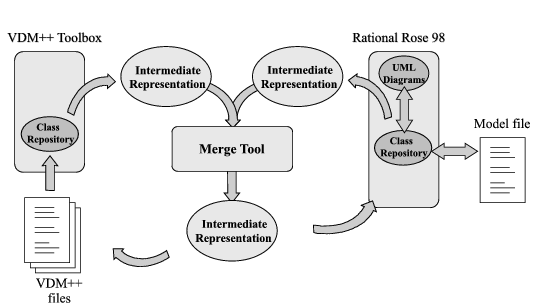
\includegraphics{vppuml_arch}}
\caption{\link{}の構造 \label{fig:architecture}}
\end{center}
\end{figure}

図の左下方よりスタートして、 \vdmpp{} ファイル ( {\tt rtf} 形式のもの) の集合が構文分析され \vdmpp{} Toolboxのクラスリポジトリに加えられる様子が、示されている。
 \link{} は \vdmpp{} 仕様を、UMLに関連する\vdmpp{}の部品である中間表現形(Intermadiate Representation)に翻訳する。
同様にUMLモデルも、 \rose{}のクラスリポジトリへアクセスすることで中間表現形に翻訳される。
この2つの中間表現形は ``互換性がある'' ので、比較や併合を行うことができる。
2つのモデルを1つの共通モデルとして併合したものを、\rose{}のクラスリポジトリと \vdmpp{}仕様ファイル群に戻すことで、\vdmpp{} モデルと UML モデルは同期する。
この2つの表現形は、上記のように幾通りかの方法で併合が可能であり、結果として \link{}を用いた次の3つの方法に集約される。
 \rose{} の中間表現形が存在しない場合、あるいはこの表現形を無視する選択をした場合、併合は \vdmpp{} から UMLへの全変換となる。
同様に、\vdmpp{} Toolbox からの結果としての中間表現形が存在しないか、あるいはこの表現形を無視する選択をした場合には、併合はUML から \vdmpp{}への全変換となる。
最後は、2つの表現形の併合を選択することである。

\subsection{Rose-VDM++ リンクのメインウィンドウ} \label{main}

この章では \link{}のGUI(グラフィカル・ユーザー・インターフェイス)について述べる。
\link{}は \vdmpp{} Toolbox 内でメニュー項目である {\it ツール/\link{}} を選択するかあるいは\raisebox{-1.0mm}{
\includegraphics[width=0.03\textwidth]{rose}} (\guicmd{Rose}) ボタンを押すことで、起動される。
図~\ref{fig:toolbox}がこのステップに該当する。

\begin{figure}[htb]
\begin{center}
\mbox{}
\resizebox{9cm}{!}{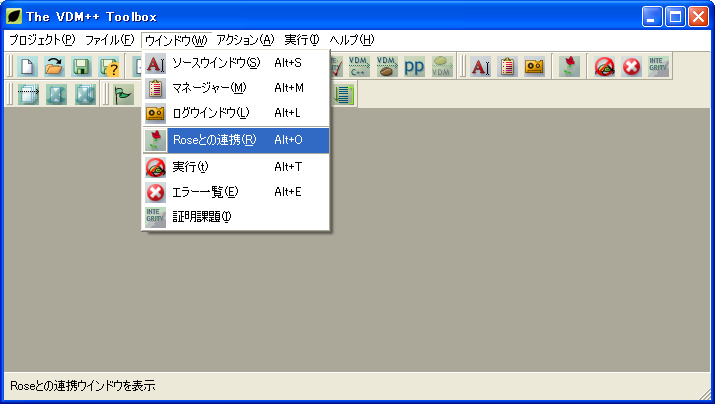
\includegraphics{invokeRose}}
\caption{\link{}の起動\label{fig:toolbox}}
\end{center}
\end{figure}

 \link{} の起動で、図~\ref{fig:userinterface}に示された別のウィンドウが開く。
起動中は、 このウィンドウから\link{}のすべての機能の操作を行うことができる。
各々のボタンの意味については、以下の章で説明していこう。

\begin{figure}[htb]
\begin{center}
\mbox{}
\resizebox{9cm}{!}{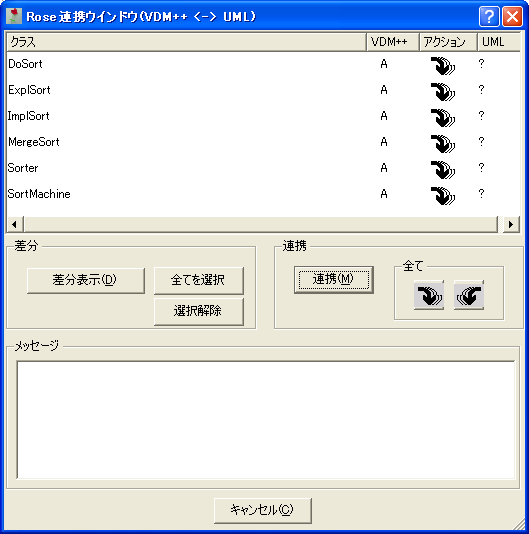
\includegraphics{roseWindow}}
\caption{\link{}のメインウィンドウ \label{fig:userinterface}}
\end{center}
\end{figure}

\link{}が起動すると、 \rose{} に対して必要とされる接続が確立される。
 \rose{} のインスタンスが既にマシン上で実行されていた場合は、 \vdmpp{} Toolbox はこのインスタンス対して接続を行う。
それ以外の場合は、 \rose{} を自動的に始動させてそのインスタンスに対して接続がなされる。
これ以降は次に挙げる簡単な規則に従って、  \link{} はRose Model Fileの読み込みを行う:

\begin{itemize}
\item \ToolboxName{}内の現プロジェクトに名前が与えられている場合(つまり、現存のプロジェクトが開いた状態、あるいは新しいプロジェクトを1つ生成し保存した状態)、 \link{} はこのプロジェクトファイルと同じ名前と配置場所をもつモデルファイルを開こうと試みる。
たとえばプロジェクトファイル {\tt MyProject.prj}に対して、 \link{} はこのプロジェクトファイルと同じディレクトリにモデルファイル  {\tt MyProject.mdl}を開こうとする。
 同じ名前のモデルファイルが存在しなければ、空のモデルファイルが生成される。
\item \ToolboxName{}中の現プロジェクトが一度も保存されていない場合でも、 \link{} はそのまま現在 \rose{}中に置かれたこのモデルを使用する。
\end{itemize}
% comment out by teramoto
%\link{} は \vdmpp{} プロジェクトファイルと共に用いることが推奨されている。
%この理由は、 \link{} はすべての {\em new} ファイルをプロジェクトファイルと同じディレクトリに生成するからである。
%常に \link{}を1つのプロジェクトファイルと一緒に用いれば、予期せぬ場所にファイルが生成されてしまうことは避けられる。
 \link{} が開始されたとき、\vdmpp{} モデルと UMLモデルの中間表現は自動的に、各々が \vdmpp{} Toolbox に含まれるクラスと\rose{}に含まれるクラスに基づき処理される。
この2つの表現形の内容は、ユーザーにクラス名称の一覧として表示され、\vdmpp{} クラスと UML クラスの各々の状態は指定の状態標識記号を用いて示される。
これら標識記号の厳密な意味の詳細は、この章の後方に記されている。
以下に続く章では、1つの表現形から別の表現形にどのように翻訳するかについて述べると共に、\link{}を用いて2つの表現形を併合する方法についても述べていく。
このツールの処理能力を描き出すために、 \cite{UserManPP-SCSK}のソートの例題を用いる。

\subsection{VDM++をUMLに変換する} \label{trans1}

 \link{} の開始前に1つ以上のクラスが構文チェックされる場合、これらのクラスは~\ref{mapping}章で述べられるマッピング規則を用いた中間表現形に翻訳されることになる。
ここで、 \vdmpp{} Toolboxの処理対象にソート例題ファイルが構成され名称 {\tt Sortpp.prj} のプロジェクトファイルが生成された、という状況を仮定してみる。
さらに \vdmpp{} ファイルの構文チェックが完了し、 \rose{}はクラス定義を含まないと仮定する。
この後に \link{} の起動を行うと、図~\ref{fig:VDMtoUML}に示されるようなクラス一覧が表示される。

\begin{figure}[htb]
\begin{center}
\mbox{}
\resizebox{9cm}{!}{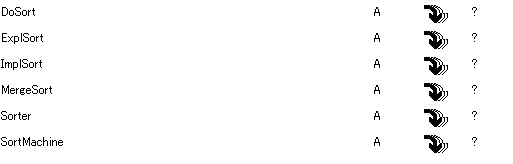
\includegraphics{sortClasses}}
\caption{ソート例に対するクラス一覧 \label{fig:VDMtoUML}}
\end{center}
\end{figure}

ここで用いられているクラス指定子は {\bf A} と  {\bf ?} で次のような意味をもつ: 

\begin{description}  
\item [A]       モデルの直前の処理でこのクラスが追加されたことを示す。
\item [?]       モデル内でこのクラスは認識されないことを示す。
\end{description}  

したがって図~\ref{fig:VDMtoUML} のクラス一覧は次のように解釈すべきである: 6つのクラスすべてが\vdmpp{} モデルに追加された。
一方 \vdmpp{} で定義されたクラスはいずれも UML モデルで認識されない、この理由は簡単で \rose{} は \link{}の起動前にクラス定義を含まないと仮定してあったからである。
一覧では各々のクラスが、2つの表現形の併合をどのように引起すかの構成に用いる独自の作用ボタンをもつ。
\link{}ウィンドウが開かれるときに、各々のボタンには結合する2つのクラス指定子に基く既定の行動が割り当てられている。
作用ボタンの状態の変更には単にクリックすればよい。
クリックで、最大4通りの異なる状態間での切り替えがなされる:

\begin{list}{}{}
\item[\resizebox{1cm}{!}{
\includegraphics{button1rosemanual}}] {\bf
    \vdmpp{} から UML:} この動作は、 \vdmpp{}で定義されたクラスの定義をUMLの同じ名クラスへマップする。
このクラスがUMLに既に存在していた場合はこれが更新され、そうでない場合は新しいクラスが生成される。
\item[\resizebox{1cm}{!}{
\includegraphics{button2rosemanual}}] {\bf UML から \vdmpp{}:} この動作は、UMLで定義されたクラスの定義を\vdmpp{}の同じ名のクラスにマップする。
この動作で、UMLで定義されたクラスの定義は\vdmpp{}の同じ名のクラスにマップされる。
結果は、新しいクラスの生成かあるいは既に存在する同じ名の\vdmpp{}クラスの定義更新となる。
第~\ref{trans2}章を参照のこと。
\item[\resizebox{1cm}{!}{
\includegraphics{button3rosemanual}}] 
{\bf 併合:} この動作は、\vdmpp{}で定義されたクラスの定義をUMLで定義されたクラスの定義に併合する。
第~\ref{merging}章を参照のこと。
\item[\resizebox{1cm}{!}{
\includegraphics{button4rosemanual}}]
{\bf 除外:} これは処理対象の新しいモデルからこのクラスを除外する。
結果は、このクラスがUMLモデルと \vdmpp{}モデルの両方から取り除かれる。
 
\end{list}


図~\ref{fig:VDMtoUML}の例において、すべての動作ボタンは既定の動作として、\vdmpp{}からUMLへのマップとして設定される。
動作ボタンのひとつをクリックすると、``\vdmpp{} から UML''と``除外'' の2つの状態が切り替え可能としてのみ現れる。
この理由は、他の2つの状態は\rose{}で定義されたクラスがないため意味がないからである。
動作ボタンの状態が変化してしまったら、``既定''ボタンをクリックすることでいつでも元の既定の設定に戻すことができる。
さて例題にもどり: \link{} に \vdmpp{} からUMLへの変換を行わせるために、 ``連携''と書かれたボタンをクリックする。
 \link{} はここで新しく6つのクラスを\rose{}のクラスリポジトリに追加する。
\link{}により生成された新しいクラスはすべて、 ``Generated classes''という名のパッケージに追加される。
しかしいつでも、 ``Generated classes''パッケージから別のパッケージに移すことは可能である。
このクラスがその後 \link{} によって更新/修正されれば、``Generated classes''パッケージに戻されることはない。
図~\ref{fig:classrepository} は、ソート例題の \vdmpp{} クラスをUMLに翻訳した後の、クラスリポジトリのスナップショットである。

\begin{figure}[htb]
\begin{center}
\mbox{}
\resizebox{6cm}{!}{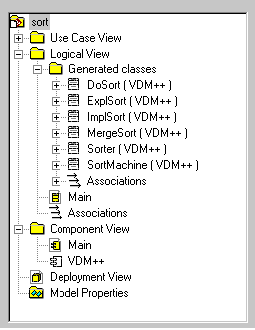
\includegraphics{classRepository}}
\caption{ソート例題に対する\rose{}のクラスリポジトリ \label{fig:classrepository}}
\end{center}
\end{figure}

1つの例として、 \vdmpp{}クラス {\tt Sorter}に対して生成されたUMLクラスを見よう。
図~\ref{fig:SorterVDMUML} はSorterクラスの\vdmpp{} 仕様と生成されたUMLクラスである。
見ての通り、このクラスの変換は極めて直接的である。
使用されるマッピング規則の詳細は、第~\ref{mapping}章を参照のこと。


\begin{figure}[htb]
\begin{center}
\hspace{-1.5cm}
%\begin{minipage}[t]{2in}
\resizebox{7cm}{!}{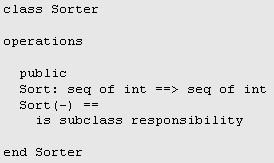
\includegraphics{sortervdm}}
%\end{minipage} \ \
%\begin{minipage}[t]{3in}
\hspace{0.2cm}
\resizebox{6cm}{!}{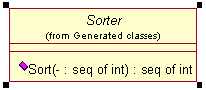
\includegraphics{sorteruml}}
%\end{minipage}
\caption{\vdmpp{} {\tt Sorter}クラス (左) と UML {\tt Sorter} クラス (右) \label{fig:SorterVDMUML}}
\end{center}
\end{figure}

 \rose{} では、クラスリポジトリを閲覧し、属性や操作の定義を検索や修正できる。
 さらに、クラスリポジトリにあるクラスからクラスダイアグラムの生成を行うことができる。
第~\ref{rose98} 章では、簡単に \rose{}の紹介を行おう。

\subsubsection*{生成されたファイル}

\rose{} のUMLモデルを更新する前に、 \link{} は現在の UML モデルのバックアップを生成している。
バックアップは、{\tt \_old} を \rose{}の現在のモデルの名前に付け足した名を用いる。
たとえば、モデルファイルである {\tt MyProject.mdl} は {\tt  MyProject\_old.mdl}にバックアップがとられる。
\vdmpp{} から UML へのマッピングが予期しない結果である場合、 \link{}でなされた変更はこのバックアップで簡単に取り戻すことができる。


\subsection{UML から VDM++への変換 } \label{trans2}
   

この章では、\rose{}で定義されたUMLモデルから \vdmpp{}を生成するため \link{} をどのように使用するかを述べる。
事柄をできる限り単純化し、第~\ref{trans1}章で生成されたモデルから \vdmpp{}を生成する。\vdmpp{} Toolboxがモデルをまったく含まない、つまり、 \link{}の発動に先立ち構文がチェックされたクラスはないということを、仮定する。
\vdmpp{} Toolboxのメニュー項目の {\it プロジェクト/新規プロジェクト} を選択し、それまでに\vdmpp{} Toolboxから持ってきたクラスをすべて削除する。
%続けて、この(空の)プロジェクトを空のディレクトリに保存し、例題に戻る
%\footnote{その中にファイルが1つも構成されていないにもかかわらずプロジェクトを保存する理由は、新しいファイルが生成された場所で制御されることが可能だからである。}。
メニュー項目の {\it Tools/\link{}}を選択すると、図~\ref{fig:UMLtoVDM} で示されたクラス一覧が表示される。
予想通り6つのクラスはどれもが \vdmpp{}では認識されないクラスで、UMLで定義されたものと分かる。

\begin{figure}[htb]
\begin{center}
\mbox{}
\resizebox{8cm}{!}{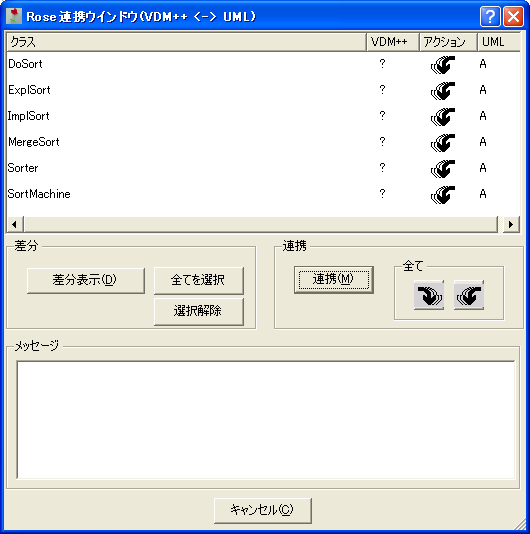
\includegraphics{classListUml}}
\caption{UML クラスのみに対するクラス一覧 \label{fig:UMLtoVDM}}
\end{center}
\end{figure}

\newpage

 ``連携'' ボタンをクリックすると、作業ディレクトリの選択ダイアログが表示される。
UMLで定義された6つのクラスに対して生成される、 \vdmpp{} クラスファイルを保存するディレクトリを選択することができる。

\begin{figure}[!htb]
\begin{center}
\mbox{}
\resizebox{9cm}{!}{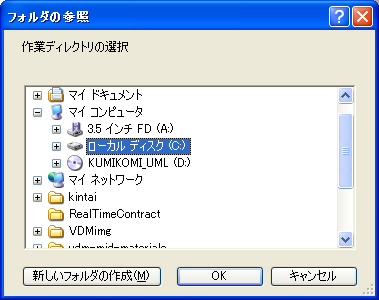
\includegraphics{seldir}}
\caption{作業ディレクトリの選択ダイアログ \label{fig:selectDirectory}}
\end{center}
\end{figure}

例として、図~\ref{fig:ExplSortVDMUML} でクラス{\tt ExplSort}のUML版と、同クラスに対して生成された \vdmpp{} 仕様、を示す。
関数機能や演算は単にシグニチャとして生成されることに注意しよう−ユーザーはそれらの本体を後で指定しなければならない。


\begin{figure}[htb]
\begin{center}
\mbox{}
\resizebox{6.5cm}{!}{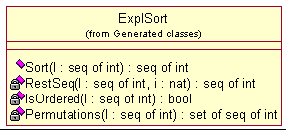
\includegraphics{explSortUml}}
\hspace{0.2cm}
\resizebox{7cm}{!}{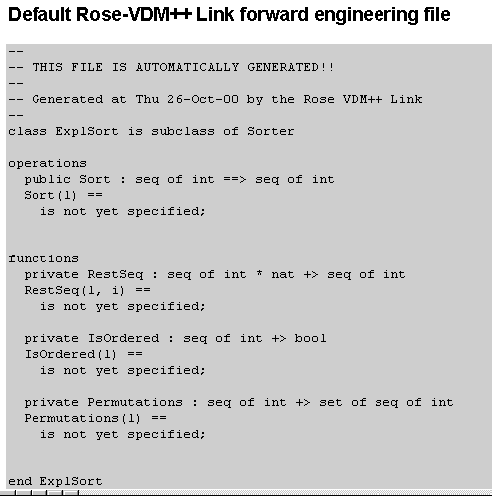
\includegraphics{explSortVdm}}
\caption{UML {\tt ExplSort} クラス (左) と \vdmpp{} {\tt ExplSort} クラス (右) \label{fig:ExplSortVDMUML}}
\end{center}
\end{figure}

\subsubsection*{生成されたファイル}

UMLに導入される新しいクラスは、各々そのクラスと同じ名前の別々の {\tt  rtf}ファイルの中に生成される。
たとえばクラス{\tt MyClass} は、プロジェクトファイルと同じディレクトリ中の {\tt  MyClass.rtf} という名前のファイルに生成される。
この名前のファイルがすでに存在する場合は、\link{} が警告を出し新しいファイルは {\em 生成されない}。
この場合は既存ファイルを移動するか名前変更をするかしておくべきで、あるいはUMLに導入されるクラスに名前の不一致を避けて他の名前を与えるべきである。
\vdmpp{} Toolbox のログウィンドウは、生成ファイルの名前すべてをディレクトリと共に表示する。
UMLに導入されるクラスに対する新しい {\tt rtf}ファイルを生成するとき、\link{} は {\tt NewClass.rtf} という名前の特別なファイルをこの新しいファイルの ``スケルトン''に用いる。
このファイルは、\ToolboxName{} インストールを行った場所の{\tt uml}サブディレクトリに {\em 置かれていなければならない}。
 このスケルトンファイルの内容は変更してもよいが、次の項目を満たすことが要求されている:

\begin{itemize}
\item 文書は {\em 常に}  VDM ブロックを、少なくとも1つの (空の可能性もある)  {\tt VDM}スタイルの段落を含む。
\item ファイル名は {\tt NewClass.rtf} である必要があり、このファイルは\ToolboxName{} インストールにおける {\tt uml} サブディレクトリに置かれている。
\end{itemize}


\subsubsection*{生成されたクラスの利用}

生成された \vdmpp{} クラスは、自動的に現在のプロジェクト加えられ構文解析が行われる。
これが可能なのは、 \link{} が常に構文的にほとんど正しいクラスを生成しているからである。
しかしながら、 Rose モデルの構文エラーは VDM++ モデルまで持ち越される (通常はキーワードの不適切な使用とされる)。
ここでおそらく、たとえば演算操作と関数機能の本体を書くというように\vdmpp{} 仕様を拡張することで、続行されることになる。
 このモデルのオブジェクト指向面(継承や関連といった関係)で修正したい、あるいは新しいインスタンス変数、関数、その他の追加が必要となった、という場面も想像される。この場合、単に生成された {\tt rtf} ファイルを編集すればよい。
その後両モデルの一貫性を保つために、新しい \vdmpp{} モデルも簡単にUMLにリバース・エンジニアリングできる。
\vdmpp{} モデルの修正を行う間はUMLモデルを変更しないという条件下で、クラスを構文チェックし(必要ならば型チェックもして)第~\ref{trans1}章の記述のように続行される。

\subsubsection*{UMLから \vdmpp{}へ変換する間に起こされる警告}


UML クラスが \vdmpp{}に翻訳されるとき、 UML 属性と演算は \vdmpp{} 構築要素に転換される。  
 UML モデルで使用された名前と型も、 必然的に\vdmpp{}の構文規則に従わなければならない。
これが当てはまらない場合は、 UML 定義は単に無視されユーザーには警告という通知がなされる。
これは、生成される \vdmpp{}仕様を構文的に最大限正しくするためである。
\link{} が UMLからの定義を読み取るときに生成される警告に対しては、注意が必要だ。なぜなら、警告が発せられるのは常にUMLモデル中で \vdmpp{}に翻訳されないものがあるからで、それは結果として構築された共通表現形において無視されてしまうことになる。 \link{} 構造の結果(第~\ref{architecture}章を参照) 、マージツールで処理された表現形は \rose{}のクラスリポジトリの現モデルを置き換える。 
UMLモデルの読み込み中に無視された構築要素は、 ``連携'' ボタンがクリックされたら除外されることを意味する。

詳しくは付録~\ref{warnings}を参照のこと。

\subsection{VDM++モデルと UML モデルの併合} \label{merging}


第~\ref{trans1}章と~\ref{trans2}章で、モデルは \vdmpp{} と UMLのどちらかで表現されたものと仮定していた、つまり、図~\ref{fig:architecture}の2つの表示のうちの1つは空であった。
これは事柄をできる限り単純に扱うためであり、また1つの表現形のモデルをもう1つの表現形に翻訳することがどのように可能かを描くためであった。
これは、既存の\vdmpp{} 仕様を記述するのにUMLダイアグラムを生成するとき、また既存のUMLモデルから\vdmpp{} を生成するときに役に立つ。
しかしもっと大きくもっと複雑なシステムをモデル化する場合、UMLと \vdmpp{}モデルが同時的に展開されるものであれば、第~\ref{trans1}章と~\ref{trans2}章の仮定は保持されるものではない。
この場合の要求に応えるため、 \link{} はこの章で2つの異なるモデルを1つに併合する機能を提供する。
以降は、\vdmpp{} Toolboxに第~\ref{trans1}章のソート例が初期化構成され、さらにこの仕様は第~\ref{trans1}章に記述されているようにUMLに翻訳されている、と仮定するとしよう。
続いて \vdmpp{} 仕様と UML モデルの両方とも少しだけ修正がなされている。

図~\ref{fig:mergeUMLVDM} で、\vdmpp{} モデルと UML モデル両方にいくらか変更がなされた後の \link{} のクラス一覧を示している。

\begin{figure}[htb]
\begin{center}
\mbox{}
\resizebox{9cm}{!}{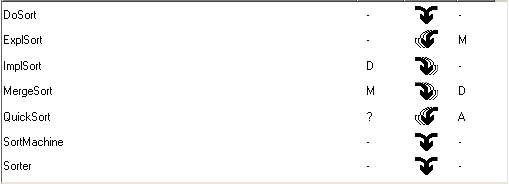
\includegraphics{bothChanged}}
\caption{UML と \vdmpp{} の両方が変更されたときのクラス一覧 \label{fig:mergeUMLVDM}}
\end{center}
\end{figure}

この図より、 UML で新しいクラス {\tt QuickSort}が追加され、 {\tt ExplSort}クラスは変更されたということが見て取れる。
さらに、 {\tt MergeSort} クラスはモデルから削除されている。
\vdmpp{} では、{\tt MergeSort} クラスが変更され {\tt ImplSort} クラスが削除されている。

図~\ref{fig:mergeUMLVDM} では {\bf M}、 {\bf -}、 {\bf D}という新しく3つのクラス指定子を紹介していて、これらは前で述べた2つの指示子と共に、 \link{}で使用される5種類のクラス指示子を構成している。
 
3つのクラス指示子は次の意味をもつ:

\begin{description}  
\item [M] はクラスが変更されたことを示す。
\item [-] はクラスに変更がないことを示す。
\item [D] はモデルが最後に実行された以降にクラスが削除されたことを示す。
\end{description}  

同じクラスで2つの表現形間の違いを調べるのに、簡単なことでクラスの横のチェックボックスをクリックし、続けて``差分''ボタンをクリックしてみる。
結果はログウィンドウに表示される。
\vdmpp{} と UML の表現形の違いをすべて調べるためには、 全クラスを選択するための``All'' ボタンを押せばよい。
図~\ref{fig:diffs} で全クラスの\vdmpp{} と UMLの表現の違いを処理した結果を示している。
たとえば、 {\tt ExplSort} クラスの2つのバージョンで関数{\tt RestSeq}に対する1つの引数の名称が異なる; ``{\tt i}''が ``{\tt j}''となっている、それのみ違うことがわかる。

\begin{figure}[htb]
\begin{center}
\mbox{}
\resizebox{9cm}{!}{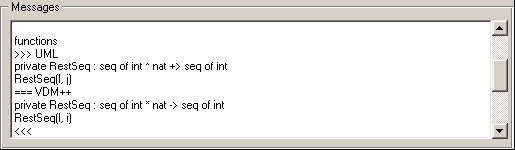
\includegraphics{differences}}
\caption{すべてのクラスに対する\vdmpp{} と UML 表現の違い \label{fig:diffs}}
\end{center}
\end{figure}

仮にこれらの2つのモデルを1つの表現形に併合したい場合、\rose{}におけるクラスリポジトリと\vdmpp{}仕様を含む {\tt rtf} ファイルに影響が及ぶ。
2つの表現形の併合をどのように行うのか決定するためには、求める動作をアクションボタンの状態を変えることで選択しなければならない。

クラス別に可能な動作の一覧を図~\ref{tab:actions} に示す。

\begin{figure}[ph]
\begin{center}
\mbox{}\vspace*{-1ex}
\begin{tabular}{|l|l|p{10cm}|} \hline
  クラス            & 可能な動作   &  ``連携'' ボタンを押した結果 \\ \hline 
\hline
DoSort             & \resizebox{1cm}{!}{
\includegraphics{button3rosemanual}} (既定)& どちらのモデルにおいてもクラスの変更はないため、更新はされない。\\
                   & \resizebox{1cm}{!}{
\includegraphics{button1rosemanual}} & 既定動作と同じ\\ 
                   & \resizebox{1cm}{!}{
\includegraphics{button2rosemanual}} & 既定動作と同じ\\
                   & \resizebox{1cm}{!}{
\includegraphics{button4rosemanual}} & クラスは両モデルから除外される。\\ \hline
Sorter             & \resizebox{1cm}{!}{
\includegraphics{button3rosemanual}} (既定)& どちらのモデルにおいてもクラスの変更はないため、更新はされない。\\
                   & \resizebox{1cm}{!}{
\includegraphics{button1rosemanual}} & 既定動作と同じ\\ 
                   & \resizebox{1cm}{!}{
\includegraphics{button2rosemanual}} & 既定動作と同じ\\
                   & \resizebox{1cm}{!}{
\includegraphics{button4rosemanual}} & クラスは両モデルから除外される。\\ \hline
ExplSort           & \resizebox{1cm}{!}{
\includegraphics{button2rosemanual}} (既定) & UMLモデルでなされた修正が \vdmpp{} モデルにおいてもなされる。\\
                   & \resizebox{1cm}{!}{
\includegraphics{button1rosemanual}} & UMLモデルでなされた修正は削除される。クラスは元の状態に戻る。\\ 
                   & \resizebox{1cm}{!}{
\includegraphics{button3rosemanual}} & 以下に述べるように矛盾がおきる。 \\
                   & \resizebox{1cm}{!}{
\includegraphics{button4rosemanual}} & クラスは両モデルから除外される。\\ \hline
ImplSort           & \resizebox{1cm}{!}{
\includegraphics{button1rosemanual}} (既定) & クラスはUMLモデルからも削除される。 \\ 
                   & \resizebox{1cm}{!}{
\includegraphics{button2rosemanual}} & 新しい ImplSort クラスが \vdmpp{} モデルに生成される。\\
                   & \resizebox{1cm}{!}{
\includegraphics{button4rosemanual}} & 既定動作と同じ\\ \hline
MergeSort           &
\resizebox{1cm}{!}{
\includegraphics{button1rosemanual}} (既定) & \vdmpp{}モデルでの変更を含む新しい MergeSort クラスが UML モデルに生成される。 \\ 
                   & \resizebox{1cm}{!}{
\includegraphics{button2rosemanual}} & クラスは \vdmpp{} モデルからも削除される。\\
                   & \resizebox{1cm}{!}{
\includegraphics{button4rosemanual}} & クラスは \vdmpp{} モデルからも削除される。\\ \hline
QuickSort          & \resizebox{1cm}{!}{
\includegraphics{button2rosemanual}} (既定) & クラスは \vdmpp{} モデルに追加される。\\
                   & \resizebox{1cm}{!}{
\includegraphics{button4rosemanual}} & クラスは両喪出るから除外される。\\ \hline
SortMachine             & \resizebox{1cm}{!}{
\includegraphics{button3rosemanual}} (既定)& どちらのモデルにおいてもクラスの変更はないため、更新はなされない。\\
                   & \resizebox{1cm}{!}{
\includegraphics{button1rosemanual}} & 既定動作と同じ\\ 
                   & \resizebox{1cm}{!}{
\includegraphics{button2rosemanual}} & 既定動作と同じ\\
                   & \resizebox{1cm}{!}{
\includegraphics{button4rosemanual}} & クラスは両モデルから除外される。\\ \hline
\end{tabular}
\caption{\vdmpp{} モデルと UML モデルの併合時に可能な動作 \label{tab:actions}}
\end{center}
\end{figure}


\subsubsection*{矛盾する定義を含むマージクラス}
\label{mergingclasses}
 
 UML モデルと \vdmpp{} モデルが平行して展開することが許される場合は、矛盾の可能性が生じる。
たとえば、 \vdmpp{}モデルと UML モデルの両方で同じ名前で異なるシグニチャを持つ操作を定義したとすると、 Merge Tool は2つのうちのどちらの操作を結果としてのモデルに選ぶべきかわからなくなる。
``連携''ボタンのクリックで2つのモデルの併合が始まるが、矛盾に出会うと併合は異常終了し、ユーザーには矛盾の起きたクラス間についての情報が届けられる。
 {\tt ExplSort}クラスの\vdmpp{}表現形と UML 表現形の併合では、たとえば両モデルの{\tt RestSeq}関数の引数の名前が1つ異なっているということから、矛盾がひき起こる。
この矛盾は図~\ref{fig:diffs}でも明らかである。
ユーザーは通常 ``Diff'' ボタンを使用して矛盾の箇所を特定し、単純に2つの定義のどちらを残すか決定する。
すべての矛盾が解決すると、 \vdmpp{} 仕様は構文チェックされ、2つのモデルの併合を行うため \link{} が再起動される。
ユーザーは矛盾を避けるためモデルの1つを変更するという代わりに、矛盾を解決するために併合モードの変更を選択することもできる。
ただ異なる状態間の切り替え用トグルボタンをクリックし、表現形の2つのうちの1つを抑制する動作を選択する。
矛盾は、表現形が併合されたときにのみ起こるのである。

\subsubsection*{ \vdmpp{} 仕様の更新}
\label{updating}
  
\vdmpp{} モデルと UML モデルが互いに矛盾しなければ、 ``連携'' ボタンのクリックで、元の2つのモデルを併合した結果を含めるために \rose{}のクラスリポジトリが自動的に更新される。
同様に\vdmpp{}プロジェクトの {\tt rtf} ファイルが自動的に更新され、UMLモデルに応じてなされた変更の反映のために構文分析が行われる。
新しいクラスが導入されていれば、 第~\ref{trans2}章で述べている様に新しい {\tt rtf} ファイルとして生成される。
 \link{} は {\tt rtf} ファイルを更新する前にそのコピーを作成する。
コピーは元のファイル名に {\tt \_old.rtf} を付与した名前となる。
つまり、ファイル {\tt ExplSort.rtf} は更新前に {\tt  ExplSort.rtf\_old.rtf} にコピーされる。
以下は \vdmpp{} 仕様ファイルの更新時に適用される規則である:


\begin{description}
\item[新しい要素] は、そのクラスの先頭に追加される。
たとえば、新しいインスタンス変数はクラスで最初の {\tt instance variables} ブロックの先頭に挿入される。
 {\tt instance variables} ブロックが \vdmpp{} クラス中ですでに宣言されている場合は、そのクラスの先頭に生成される。
\item[古い要素] は、\vdmpp{} のコメントに変換されファイルから除外される。
この方法ならば、除外の必要のなかったものを簡単に元に戻すことができる。
\item[修正された要素] は、単純に古い定義を(コメント化して)除外し新しい定義を追加するという方法で扱われる。
\end{description}

仕様ファイルの修正すべては、次のコメントで識別されることになる: ``Rose-VDM++ リンクによる追加'' あるいは ``Rose-VDM++ リンクによる削除''。
図~\ref{fig:update} は、 関数{\tt  RestSeq}のシグニチャがUMLで修正された結果、\link{} によって{\tt ExplSort}クラスがどのように更新を受けたかを表している。
ある状況下で \link{} が必要なファイルの更新ができなくなることがある。
一部のワードプロセッサーでは、今編集中のファイルはロックすることで他のアプリケーションからのアクセスを許可しない。
この結果として \link{} はロックされたファイルを更新することができない。
更新するべきファイルが他のアプリケーションによりロックされていれば、 \link{}はそれらのファイル名称を一覧にし、ユーザーは(他のアプリケーションがこれらを使用中でないことを確認することで)ロックを解除するかまたは併合処理をキャンセルするか、どちらか選べる。
\link{}で修正されるすべてのファイルは、\ToolboxName{}のモデルが \rose{}のモデルと同一になるように、それ以降は自動的に構文解析される。

\begin{figure}[htb]
\begin{center}
\mbox{}
\resizebox{11cm}{!}{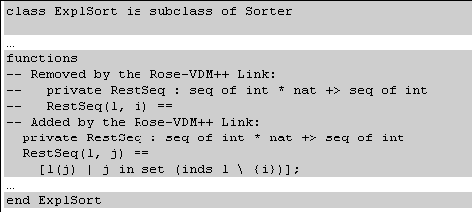
\includegraphics{updatedRtf}}
\caption{更新された {\tt ExplSort.rtf} ファイル \label{fig:update}}
\end{center}
\end{figure}


\subsection{仕様の型チェック} \label{sec:typecheck}

 \link\ を用いるために、 \vdmpp\ 仕様は唯一構文チェックのされる必要があるが、同様に型チェックも推奨されている。
インスタンス変数で定義されたクラス間関係の情報は、仕様が型チェックされるまで利用できない。
したがって \vdmpp\ 仕様がただ構文チェックのみされていた場合、このような関係で定義され、関連生成ができないという意味で \link\ は完全とは言えないかもしれない。

\newpage  
\section{Rational Rose} \label{rose98}
  
ここまでで\link{}の特徴のいくつかを論じてきた。
このツールは\rose{}との密接な結び付きに依存するため、このマニュアルの適用範囲として\rose{}へ簡単な導入を行う。
最初に、\link{}によって生成されたクラスやユーザーが生成したクラスから、クラスダイアグラムを作る方法を述べる。
第~\ref{manipulate}章は \rose{}で定義の修正、削除、追加を行う方法が述べられている。
 \link{} はいわゆる\rose{}のアドイン言語であり、~\cite{InstallPPMan-SCSK}で述べられているようにインストールできる。 
このアドインは \rose{}のアドインマネージャーを通した起動や終了が可能である。
 \rose{}は \link{} の起動(既定で起動)で、 \vdmpp{}、 \vdmpp{} の基本データ型とUMLから\vdmpp{}へのマッピングで使用される特殊なステレオタイプ、を 認識する。

\subsection{Rational Roseにおけるクラスダイアグラム} \label{diagrams}
  
\subsubsection*{クラスダイアグラムの生成}

 \vdmpp{} クラス定義を UML に翻訳するのは、\rose{}のクラスリポジトリにおけるクラス定義を単に作成または更新するということで−自動的にクラスダイアグラムの生成は行わない。
しかし、 \rose{} ではクラスダイアグラムの生成は簡単である。
 \rose{}でクラスダイアグラムを生成するには、次のように進める (以下の動作は \rose{}内から行う):


\begin{enumerate}  
\item 空のクラスダイアグラムを作成するか、既に存在するものを開く。
\item クラスダイアグラムにクラスを追加する 
\begin{itemize} 
\item ドラッグアンドドロップ: クラスリポジトリ中のクラスを1つクリックし、それを追加したいクラスダイアグラム中にドロップする。
\item  {\it Query/Add Classes...}を選択し、追加したいクラスを含むパッケージ(通常は "生成クラス" パッケージ)を選ぶ 。   
 "選択クラス" リストボックスに追加するクラスを移動し、"OK"をクリックする。
選択済みクラスはすべて自動的に作動中のダイアグラムに追加され、自動的にダイアグラムに配置される。
\end{itemize}
\end{enumerate}

図~\ref{fig:classdiagram} で、このアプローチにより生成されたクラスを示す。

\begin{figure}[htb]
\begin{center}
\mbox{}
\resizebox{9cm}{!}{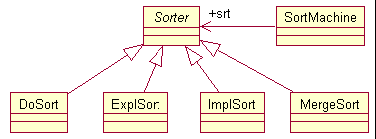
\includegraphics{classDiagram}}
\caption{ソート例についての\rose{} のクラスダイアグラム \label{fig:classdiagram}}
\end{center}
\end{figure}

\subsubsection*{ダイアグラムの修正}

\rose{}は生成されたダイアグラムの配置変更も行う。
マウスを用い簡単な操作で、クラスや関連を他の任意のクラスに移そう。
\rose{}のクラスダイアグラムを修正すると以下の影響がある:  

\begin{itemize}
\item 配置替えで、つまりクラスや関連の移動でそのダイアグラムに修正が行われるが、クラスリポジトリへの影響はない。
さらに後で、\link{} がリポジトリを更新する場合も、ダイアグラムの配置は変えない。
クラスがリポジトリから削除されたときだけは、あるいは他のクラスに対して関連が変化したときは、ダイアグラムの表示が変化するであろうが、レイアウトの原型は保たれる。
\item クラス間に関係(継承か関連)を追加することで、クラスリポジトリのクラス定義は変化する、つまり、モデルに新しい関係が追加される。
新しい関係が追加されたダイアグラムは当然すぐに形を変える。
それに対し、他のダイアグラムは新しい関係を示すことはないが、変化を反映する更新はなされているはずである。
次の章ではクラスダイアグラムの更新方法を述べる。
\item クラスのインスタンス変数、演算、その他の変更は、クラスを含む他のすべてのダイアグラムですぐに表示される。
\end{itemize}

\subsubsection*{関係の選別}
 
\rose{} は、選択中のダイアグラムである種の関係の型を残すという機能を提供している。
この機能を用いて、クラス間の継承関係のみが示されるようなダイアグラムを簡単に構築することができる。
 \rose{}でどのような種類の関係をダイアグラムに表示するかを指定するために、 {\it Query/Filter relationships...} を選択する。
%Figure~\ref{fig:relations} shows the dialogue box for filtering relations.  
図~\ref{fig:relations} では、関係選択のためのダイアログボックスを示している。

\begin{figure}[htb]
\begin{center}
\mbox{}
\resizebox{7cm}{!}{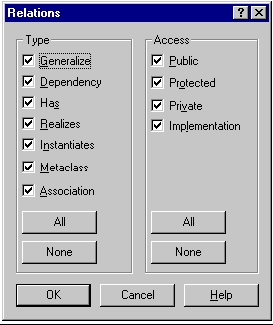
\includegraphics{relations}}
\caption{関係の指定 \label{fig:relations}}
\end{center}
\end{figure}

このダイアグラムボックスは、ダイアグラムの関係の更新にも使用できる。
単純に全種類の関係を選択し (``All'' ボタンを使用) 、 ``OK''をクリックしよう。
すると現在選択されたクラスダイアグラムのクラス間で定義された全関係が、再表示される。
\link{}により追加されて既存のダイアグラムに表示された新しい関連を確定する、ただ1つの方法である。

\subsubsection*{ローカルビュー}


しばしば単一のクラスダイアグラムで、すべてのクラスとそれらの相互関係を示すのにあまりに複雑になりすぎて、結果として理解するのが困難になる場合がある。
この理由から \rose{} では、ローカルビューの生成機能を提供する。
このため、始めに初期状態としてローカルビューを作成する対象の1つ以上のクラスから構成される新しいクラスダイアグラムを作成することが必要で、これに対してローカルビューを作成したいと考える。
後はこの新しいダイアグラムでクラスを選択し、 {\it Query/Expand Selected  Elements...} メニュー項目を選ぶ。
ダイアグラムウィンドウが飛び出し、生成するローカルビューで見たいレベル番号と関係を決定するよう促される。
 ``OK'' ボタンをクリックすれば、生成されるローカルビューを見せるクラスダイアグラムの作成が行われる。

この処理を用いて、たとえばクラスとそのすべての直接のスーパークラスとサブクラスを表示する新しいクラスダイアグラムの生成が、簡単に行える。

\subsection{Rational Roseにおける操作定義} \label{manipulate}
  
\rose{}においては常に、任意の定義の修正、削除、追加が許される。
この章では、Rose モデルの変更を行う例をいくつか挙げる。

\subsubsection*{リポジトリ内の定義の修正}
  
\rose{}における属性の定義 (\vdmpp{}においてはインスタンス変数と値) および操作 ( \vdmpp{}においては操作と関数) は、簡単に修正できる。
修正したいクラスをダブルクリックするという簡単な操作で、ダイアログボックスが現れ、クラスのすべての部位に対する定義を検証し変更する機能が提供される。
``クラス仕様''ウィンドウは任意クラスの仕様の閲覧に用いられる。
図~\ref{fig:classspecification}は、 {\tt SortMachine} クラスの仕様ウィンドウを表示している。

\begin{figure}[htb]
\begin{center}
\mbox{}
\resizebox{7cm}{!}{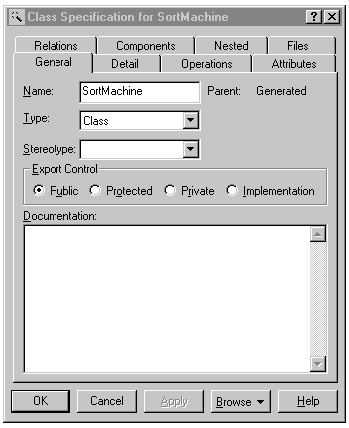
\includegraphics{sortMachineClass}}
\caption{クラス {\tt SortMachine}に対するUMLクラス仕様 \label{fig:classspecification}}
\end{center}
\end{figure}

\subsubsection*{特定の実体型の生成}
  
ここで、 \rose{}では新しい実体がどのように生成されるかを述べよう。
UMLの実体は \vdmpp{}構築要素にマップできるが、これ以上のことは第~\ref{mapping}章を読むことをお勧めする。
\rose{}の \vdmpp{}アドインが、新しい実体を生成する際の助けをする。
以下では、クラス、属性、演算、関連、の生成について述べていこう。

\begin{itemize}
%\item{\bf Classes} 
\item{\bf クラス} 

\rose{}の \resizebox{1cm}{!}{
\includegraphics{button5rosemanual}}ボタンを選択することで、新しいクラスが生成される。
基本的な \vdmpp{} 型や \link{} で定義済みのステレオタイプを使用するためには、 \vdmpp{} コンポーネントとして新しいクラスが 割り当てられなければならない。
このために、次の手順に従う:

  \begin{itemize}
  \item \rose{}のブラウザで``Component  View'' パッケージを右クリックし新しいコンポーネントを作成してから、 {\em  New/Component}を選択する。
この新しいコンポーネントをダブルクリックし、その仕様ウィンドウ (``General'' タブ上)の言語に \vdmpp{} を選ぶ。
  \item この新しいコンポーネントの仕様ウィンドウ内で``Realizes'' タブを選択して、割り当てるべきクラスを選択する。
それら選択クラスは右クリックし ``Assign''を選ぶことで、 \vdmpp{} コンポーネントに割り当てられる。
  \end{itemize}

もう1つの方法としては、マウスでクラスをドラッグしコンポーネントの中に入れることで、簡単にこれらのクラスのコンポーネント割り当てを行うことができる。

\item{\bf 属性}

 第~\ref{mapping}章で述べたように、 UML の属性は\vdmpp{}のインスタンス変数と値を表現するために用いられる。
クラスを右クリックしメニュー項目{\it New Attribute}を選択すれば、そのクラスに簡単に 新しい属性を追加できる。 
 第~\ref{mapping}章で述べているが、 3種の\vdmpp{}構造を区別するために{\it ステレオタイプ}を使う。
各々の属性に対しては、ステレオタイプ (``{\tt <<}'' ``{\tt >>}''で指定) を割り当てることができる。
ステレオタイプを指定しなかった場合、属性は既定でインスタンス変数と見なされる。
 \vdmpp{} アドインが、属性に対するステレオタイプを定義する際の手助けを行う。
図~\ref{fig:stereotype} で、新しく追加された属性の``Attribute  Specification'' ウィンドウを示す。
このクラスは \vdmpp{} コンポーネントに割り当てられるため、3つの定義済みのステレオタイプの中から、{\tt <<instance variable>>}または {\tt <<value>>}を選ぶことができる。

\begin{figure}[htb]
\begin{center}
\mbox{}
\resizebox{7cm}{!}{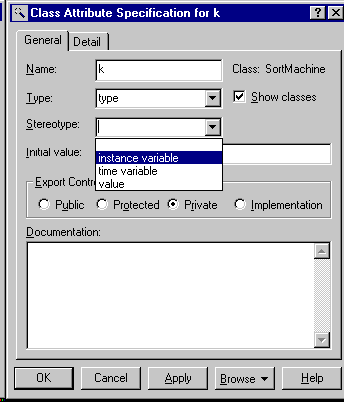
\includegraphics{stereotype}}
\caption{属性に対する定義済みステレオタイプの選択 \label{fig:stereotype}}
\end{center}
\end{figure}

\item {\bf 操作}


  クラスを右クリックしメニュー項目を選択することで、簡単に新しい操作をクラスに追加することができる。
属性で用いたと同様、 \vdmpp{}の関数と操作を区別するためにステレオタイプを用いる。
これらのステレオタイプは属性と同様にして作成される。
ステレオタイプが省略された場合は、既定ですべてが操作であると解釈される。

\item{\bf 関連}
  
2つのクラス間に関連を定義するには、 簡単なことでまず``Association Tool'' をクリックしてから、1つのクラスをクリックしマウスを他のクラスにドラッグする。
ダブルクリックすると``Association Specification''ウィンドウが開かれ、更に関連の詳細を指定できる。
ここでは関連に対する、ロール名、多重度、制約、を追加することができる。

\begin{description}
\item [ロール名:] マッピング規則で述べたが、関連のロール名は、関連の翻訳対象となるインスタンス変数の名前として用いられる。
このため関連に少なくとも1つのロール名を与えることが、生成された \vdmpp{}クラスが1つのインスタンス変数として表されるために、極めて重要である。
ロール名が与えられていない関連は、単に無視されてしまう。
\item [多重度:] ロールに対する多重度が指定されていない場合、既定で1が仮定される。
\item [制約:]  ``Association Specification'' ウィンドウにおいては、ある関連のロールに対して複数の制約を追加することが可能である。
例えば{\tt \{ordered\}}といった制約をロールに追加すると、これが\vdmpp{}に翻訳されるとき、オブジェクト参照では{\it set} でなく{\it 配列}(sequence)が生成される。
\item [限定子:] 関連に簡単に限定子を追加できる。
  限定子を保持するためには、クラスの傍の関連を単純に右クリックし、そこで {\em New Key/Qualifier}を選択する。
\vdmpp{} 内で限定された関連をモデル化したマップ中では、定義域として用いるために限定子の名前に\vdmpp{} 型を指定する(第~\ref{mapping}章参照)。
修正するロールの傍の関連を右クリックすることで、関連に関する2つのロールの詳細をいろいろ修正することができることを覚えておこう。
\end{description}  

\end{itemize}
  
\newpage  
\section{VDM++ と UMLの間のマッピング規則} \label{mapping}
  
この章では、 \vdmpp{} と UML 間の関係を示す。
これは、 \link{} で1つの表現形から他の形に変換を行うときの適用規則を示すということになる。
以下のマッピング規則を完全に理解するためには、明らかに、 \vdmpp{}  と UML について詳細な知識が必要とされる。
ここでは2つの表記法についての紹介は行わないで、必要な場合は単に様々な構築要素について述べるに留める。
完全な提示を行うために \cite{LangManPP-SCSK} と \cite{Booch&97} を参照する。
以下の章で提示する規則は、付録~\ref{rules}の図~\ref{tab:mapping}にまとめている。
 \vdmpp{}仕様のいくつかをそれに対するUML変換と共に表示することで、規則提示とする。これと関連して、定義されたマッピングが {\it  injective}であることを述べておくことが重要で、結局 \vdmpp{} から UMLへのマッピング定義は、同時に逆マッピングの定義となる。
更には、以下の規則は \vdmpp{}で記述できるすべての構築要素を{\it 網羅するものではなく}、UMLのすべての特徴も網羅してはいない、ことを述べておくこと大切である。
マッピング規則は単にマッピングを1対1にするために定義されているので、2つの表現形のうちの1つでしか記述できない構築要素はマッピングの外に取り残されていることを意味する。
 \link{} では、以下のマッピング規則で網羅されていない構築要素は単に無視される。

\subsection{クラス構造} \label{classstructure}
  
この章では、2つの表現形の間で内部のクラス構造がどのようにマップされるのかを明らかにする。

\subsubsection*{インスタンス変数と値}
 
\vdmpp{} において、あるオブジェクトの内部状態はインスタンス変数と値定義によって叙述される。
値とインスタンス変数の主な違いは、値は読み取り専用であるということだ。
UML においては内部状態は属性部に記述されるが、ここでインスタンス変数と値をそれらに対応する型と値と共に簡単な一覧にしてみる。
 インスタンス変数と値を区別するために、 {\tt <<instance variable>>} と {\tt <<value>>}という名の {\it ステレオタイプ}を用いる。 
UMLで宣言される属性に対する構文は、次の通り:  

\begin{quote}
\begin{verbatim}
name : type = initial-value
名称 : 型 = 初期値-値
\end{verbatim}
\end{quote}

これは \vdmpp{}でのインスタンス変数と値の定義の構文とほぼ一致する。
したがって値とインスタンス変数は、UMLに直接マップされ得る。
図~\ref{fig:queue} では、インスタンス変数と値のマッピングを描く。

%\subsubsection*{Time Variables}  
%
%In \vdmpp{} real-time behaviour can be expressed through the use of time variables to   
%represent continuous functions of time. Time variables can be either input or output   
%variables, distinguished in \vdmpp{} by the optional keyword {\tt input}. At the UML level time   
%variables will be listed as attributes and distinguished from values and instance variables   
%by the stereotype {\tt <<time variable>>}. In UML adding the constraint {\tt \{input\}} to the   
%name of the time variable will identify input time variables.  
%Time variables can be subject to invariants in the same way as instance variables are, only   
%here expressed as either {\it assumptions} or {\it effects}. Assumptions apply to input variables and   
%describe the requirements the input must fulfil for the system to function properly (i.e., an   
%invariant on input variables), while effects describe the expected behaviour of output   
%variables. The mapping, however, will not consider neither the assumptions nor the effect   
%clauses.  

%\begin{figure}[htb]
\begin{figure}[p]
\begin{center}
\hspace{-2cm}
\begin{minipage}[t]{2.5in}
\verbatimfile{class.vpp}
\end{minipage} \ \
\begin{minipage}[t]{2in}
\vspace{2cm}
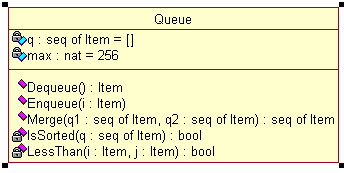
\includegraphics[width=2.8in]{queueClass}
\end{minipage}
\caption{\vdmpp{} と UML\label{fig:queue}間でクラスのマッピング \label{fig:queue}}
\end{center}
\end{figure}

\subsubsection*{操作と関数}
  
操作と関数は、UMLクラスの操作部中にマップされる。
ここでは、ステレオタイプ {\tt <<operation>>}と {\tt <<function>>}に区別される。 
UMLで操作見出しの定義を行うための構文は、次の通り:

\begin{quote}
\begin{verbatim}
名称(引数 : 型, ...) : 戻り型  
\end{verbatim}
\end{quote}
  
これは、 \vdmpp{}で陰定義関数/操作のための構文とほぼ同じである。
明示的にあるいは暗黙で定義された関数見出しは、操作見出しと同様に、この構文に変形されなければならない。
マッピングの操作と関数の例題は、図~\ref{fig:queue} を参照のこと。
操作で定義された事前条件と事後条件は、UMLマッパーに保持される。
これは、構文的に正しいVDM式として記述される必要があるからである。
 UML は操作の結果識別子の定義方法を提供しないため、特殊識別子 \textbf{RESULT}が、事後条件の中で操作結果の記述に使用される。
陽または陰関数をUMLの同じ構文にマッピングするため、UMLから\vdmpp{}へのマッピングで陰定義関数と陽定義関数の区別は難しくなる。
このため、以下の規則がUMLから\vdmpp{}への関数のマッピングに適用される:

\begin{itemize}
\item ある関数がすでに\vdmpp{}で定義されている場合、\vdmpp{}の中で定義されているのと同じ種類に(暗黙的にあるいは明示的に)マップされる。
\item ある関数が \vdmpp{}で認識されていなければ (UMLレベルで定義された関数であれば)、明示的にマップされる。
\end{itemize}

\subsection{クラス間の関連} \label{assoclasses}
  
 \vdmpp{}において、オブジェクト (クラスの実体) は、他のクラスのオブジェクトあるいはクラス自身のオブジェクトと関係をもつ可能性がある。
このようなクライアント側の関係は、オブジェクト参照型を介して可能となる。
UML ではこういった関係を関連と呼び、{\it client} クラスから参照されるクラスへ向けた矢印によって表示される。
このように矢印は\link{}の{\it 方向} を表し、オブジェクトは実際に他から参照することができる。
図~\ref{fig:classA}では、\vdmpp{} とUMLの間でこのように単純な関連付けがマップされる様子を示す。
オブジェクト参照を表すインスタンス変数はUMLクラスで属性とみなされることはない、ということは注意しよう。

\begin{figure}[htb]
\begin{center}
\hspace{-2cm}
\begin{minipage}[t]{2in}
\begin{verbatim}
class A  
instance variables  
  a: A;  
  b: B;  
  c: C;  
end A  
  
class B  
end B  
  
class C  
instance variables  
  a: A;  
end C  
\end{verbatim}
\end{minipage} \ \
\begin{minipage}[t]{2in}
\vspace{1cm}
\resizebox{8cm}{!}{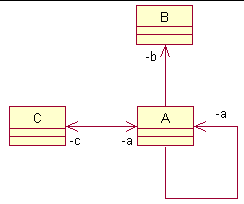
\includegraphics{refs}}
\end{minipage}
\caption{\vdmpp{} と UML間でのオブジェクト参照/関連のマッピング \label{fig:classA}}
\end{center}
\end{figure}


\renewcommand{\textfraction}{0}
                              

\renewcommand{\topfraction}{1}
                              

\setcounter{totalnumber}{100} 
\setcounter{topnumber}{100} 
   
UML において関連の {\it far end} はロールと呼ばれる。
通常ロールには名前が与えられるが、少なくとも実社会モデルにおいては、関連の役割を記載する傾向がある。
ロールは2項関連の場合には特に役立つ。
ここで、関連を表すインスタンス変数の名前から簡単にロール名を構築してみよう。
これは図~\ref{fig:classA}においても示されている。

\subsubsection*{関連に多重度を追加}
  
ここまでは単純な ``1対1'' の関連付けを考えてきた、つまり、 1つのクラスの実体がきっちり1つの他の実体に接続する関係である。
 {\tt seq of A} や {\tt set of A}といった構築要素を用いて、1つの実体をいくつかの他の実体と関係付けることができる。
 UML においては、関連の最後に数字/記号を追加し多重度を示すことで、多重度が表現される。

ここで、関連の多重度に関係する別の \vdmpp{} 構築要素がどのようにUMLにマップされるかを示そう。

\begin{description}
\item [{\tt set of objref}:]  この構築要素は ``1対多'' の関連に翻訳されるが、UMLにおいては、関連の1端に``1''を置き多端に範囲である ``0..*''を置くことでモデル化される。
\item [{\tt seq of objref}:]  これはまた1対多の関連であり、配列型を用いることで参照に順番を与えているため、UMLでは 関連の多端に対して{ordered}の制約を追加し表示する。
\item [{\tt seq1 of objref}:]  オブジェクト参照の空でない配列は、関連の多側の範囲 ``1..*'' で表示される。  
\item [{\tt [objref]}:]  オプションのオブジェクト参照は、関連のロールに範囲 ``0..1''を追加することで識別される。
\end{description}

これらの構築要素は図~\ref{fig:classD}にまとめられている。

\begin{figure}[htb]
\begin{center}
\hspace{-2cm}\begin{minipage}[t]{2in}
\begin{verbatim}
class D  
instance variables  
  es: set of E;  
  fs: seq1 of F;  
end D  
  
class E  
instance variables  
  opt_f: [F];  
end E  
  
class F  
instance variables  
  d: D;  
end F  
\end{verbatim}
\end{minipage} \ \
\begin{minipage}[t]{2in}
\vspace{1cm}
\resizebox{8cm}{!}{\includegraphics{multiRefs}}
\end{minipage}
\caption{\vdmpp{} と UML間の多重オブジェクト参照のマッピング \label{fig:classD}}
\end{center}
\end{figure}

\subsubsection*{ {\tt map} と {\tt inmap}を用いたオブジェクト参照}


 \vdmpp{} では、オブジェクトをmap型とinmap型を用いて関係づけることができる。
\vdmpp{} は {\tt map type to objref}というように構築し、ここで {\tt  type} は任意の \vdmpp{} 型、 {\tt objref} は単一あるいは多数のオブジェクト参照で、結果として {\it 限定子つき関連}となる。

限定子つき関連の多様性もまた、関連の他の型と同様に与えられる得るものである。
 UML では限定子自体に名前を割り当てることが可能で、この場合は写像の定義域の型となる。
他の関連と同様、この関連のロール名はマップを表示するインスタンス変数の名称である。
例題として図~\ref{fig:classG} を参照のこと。

\begin{figure}[htb]
\begin{center}
\hspace{-1cm}
\begin{minipage}[t]{2.5in}
\begin{verbatim}  
class G  
instance variables  
  qual_h: map nat to H;  
end G  
  
class H  
instance variables  
  qual_j: map real to J;  
end H  
  
class J  
instance variables  
  qual_h: map nat to set of H;  
end J  
\end{verbatim}
\end{minipage} \ \
\begin{minipage}[t]{2.5in}
\vspace{1cm}
\resizebox{7cm}{!}{\includegraphics{qualifiedAssociations}}
\end{minipage}
\caption{マップを用いて定義されたオブジェクト参照からの限定子つき関連 \label{fig:classG}}
\end{center}
\end{figure}

\begin{figure}[h]
\vspace{1cm}
\begin{center}
%\hspace{-2cm}
\begin{minipage}[h]{2.5in}
\begin{verbatim}  
class Super  
operations
  methodA() ==  
    is subclass responsibility;  
  methodB() ==  
    ...;  
end Super  
  
class SubA is subclass of Super  
end SubA  
  
class SubB is subclass of Super  
end SubB  
\end{verbatim}
\end{minipage} \ \
\hspace{1cm}
\begin{minipage}[h]{2.5in}
\vspace{1cm}
\resizebox{6cm}{!}{\includegraphics{inheritance}}
\end{minipage}
\caption{\vdmpp{} と UML間の継承のマッピング \label{fig:super}}
\end{center}
\end{figure}

\subsubsection*{継承関係}
\label{inheritance}

 \vdmpp{} から UML へまたはその逆の継承の翻訳は、わかりやすい。
図~\ref{fig:super} で例題を示す。
{\tt SubA} クラスと {\tt SubB}クラス は {\tt Super}クラスから継承する。
UMLにおいて、継承関係は汎化として表示される。
  
\subsubsection*{委任}

 \vdmpp{} では操作の仕様は、 {\tt is subclass responsibility} 節を用いてサブクラスに委任することができる。
UML ではこのような操作は {\it 抽象メソッド}と呼び、抽象的な操作を含む節は {\it 抽象クラス}と呼び、具体的なクラスと対比する。
少なくともその操作の1つを委任した (少なくとも1つの操作を {\tt is subclass responsibility}を用いて指定した)場合にクラスは抽象的と見なされ、それ以外は具体的と見なされる。
 UML では抽象クラスと操作は、名前をイタリックフォントで書くことで識別される。

\bibliographystyle{alpha}
\newpage
\bibliography{ifad}  
  
\newpage
\appendix
\section{マッピング規則のまとめ} \label{rules}
図~\ref{tab:mapping}のテーブルは \link{}で適用されるマッピング規則をまとめている:  

\begin{figure}[!hb]
\begin{center}
\mbox{}
\begin{tabular}{|p{65mm}|p{8cm}|} \hline
  \vdmpp{}           & UML  \\ \hline \hline
  instance variable            & ステレオタイプ {\tt <<instance variable>>}の属性 \\ \hline
   value          & ステレオタイプ {\tt <<value>>}の属性\\ \hline
%   time variable          & attribute with stereotype {\tt <<time variable>>}. Input time variables are marked by the   
%constraint {\tt \{input\}}  \\ \hline
 operation           & ステレオタイプ {\tt <<operation>>}の操作 \\ \hline
  function          & ステレオタイプ {\tt <<function>>}の操作。
UMLでのみ定義されていて \vdmpp{}に明白な関数としてマップされた関数。
それ以外、関数は暗黙であるいは \vdmpp{}で定義済みとして明白にマップされる。
\\ \hline
  {\tt obj: OtherClass}            & \resizebox{7.9cm}{!}{\includegraphics{thisclass1}} \\ \hline
  {\tt obj: set of OtherClass}         & \resizebox{7.9cm}{!}{\includegraphics{thisclass2}} \\ \hline
  {\tt obj: seq of OtherClass}        & \resizebox{7.9cm}{!}{\includegraphics{thisclass3}} \\ \hline
  {\tt obj: seq1 of OtherClass}         & \resizebox{7.9cm}{!}{\includegraphics{thisclass4}} \\ \hline
  {\tt obj: [OtherClass]}         & \resizebox{7.9cm}{!}{\includegraphics{thisclass5}} \\ \hline
  {\tt obj: map type to OtherClass}         & \resizebox{7.9cm}{!}{\includegraphics{thisclass6}} \\ \hline
  {\tt class ThisClass is subclass}\newline {\tt of OtherClass}   & \resizebox{2.5cm}{!}{\includegraphics{thisclass7}} \\ \hline
\end{tabular}
\caption{\link{}で適用されるマッピング規則 \label{tab:mapping}}
\end{center}
\end{figure}

\clearpage

\section{Rose-VDM++ リンクにより生成される警告} \label{warnings}

図~\ref{fig:architecture}を見直してみる。 
2つのモデルを併合する前に、 \vdmpp{} と UML モデルの両方が内部表現に翻訳されている。

この翻訳はいくつか検査を含み、結果いくつか別の警告がなされる可能性がある。
%%
%% For the time being these warnings are NOT generated:
%%
%% \subsubsection*{Warnings Generated during the Translation from \vdmpp{}  to UML}
%%   
%% During the translation from \vdmpp{} to UML certain warnings may be
%% generated. As mentioned earlier, the mapping rules described in
%% Section~\ref{mapping} define how one representation is translated into
%% the other. However, if one writes a \vdmpp{} construct, which does not
%% "fit" into the defined mapping rules, the user will be notified by a
%% warning identifying the \vdmpp{} construct causing the warning.
%% 
%% The \vdmpp{} constructs causing the warnings are 
%% instance variables which are defined somehow using the object reference
%% type, but which do not ``fit'' into the
%% defined mapping rules.
%% 
%% These instance variables will be mapped to UML simply as instance variables
%% and not as associations.
%% 
%% Look at the following example:
%% 
%% \begin{quote}
%% \begin{verbatim}
%% class ThisClass
%% 
%% instance variables
%% 
%%   obj: set of seq of OtherClass
%% 
%% end ThisClass
%% 
%% class OtherClass
%% end OtherClass
%% \end{verbatim}
%% \end{quote}
%% 
%% The loading of the \vdmpp{} model will result in a warning, which can
%% be seen in Figure~\ref{fig:warningThisClass}.  Moreover, mapping the
%% \vdmpp{} specification to UML without removing the construct causing
%% the warning, will result in the UML model, shown in
%% Figure~\ref{fig:wrongUML}.
%% 
%% \begin{figure}[htb]
%% \begin{center}
%% \mbox{}
%% \vspace{0.5cm}
%% \resizebox{6cm}{!}{\includegraphics{fig18rosemanual}}
%% \caption{Warning generated when computing a UML representation for the instance variable {\tt set of seq of OtherClass}.\label{fig:warningThisClass}}
%% \end{center}
%% \end{figure}
%% 
%% \begin{figure}[htb]
%% \begin{center}
%% \mbox{}
%% \vspace{0.5cm}
%% \resizebox{6cm}{!}{\includegraphics{fig19rosemanual}}
%% \caption{The generated UML model.\label{fig:wrongUML}}
%% \end{center}
%% \end{figure}

\subsubsection*{ UML から \vdmpp{}への翻訳中に生成される警告}


 UML クラスが \vdmpp{}に翻訳される場合、 UML 属性と操作は \vdmpp{} 構築要素に転換される。
UMLモデルで使用される名称と型は、必然的に\vdmpp{}の構文上の規則に従わなければならない。
従わないものがある場合、 UML 定義は単に無視され、ユーザーは警告による注意を受ける。
これは生成される \vdmpp{}仕様の構文的正当性を最大限にするために行われる。

1つの例題として、図~\ref{fig:noncompliance}に示されるUMLクラスを見よう。

\begin{figure}[htb]
\begin{center}
\mbox{}
\vspace{0.5cm}
\includegraphics{noncompliance}
\caption{\vdmpp{}の構文規則に従わないUML クラス ( \$\ 記号をここで用いることはできない) \label{fig:noncompliance}}
\end{center}
\end{figure}

UMLモデルを取り込むときに生成される警告を図~\ref{fig:warning}で示す。

\begin{figure}[htb]
\begin{center}
\mbox{}
\vspace{0.5cm}
\resizebox{9cm}{!}{\includegraphics{warning}}
\caption{インスタンス変数の定義が \vdmpp{}の構文規則に従わない場合、警告がなされる \label{fig:warning}}
\end{center}
\end{figure}
 警告の原因となるUML定義を取り除かずにUML モデルから \vdmpp{}へマッピングを行う場合、結果は以下のような \vdmpp{} クラス定義となる:

\begin{quote}
\begin{verbatim}
class ThisClass
end ThisClass
\end{verbatim}
\end{quote}

見ての通り、生成されるクラス定義は単なる空となる。
\end{document}





